This part is responsible for doing the interpratation between the two different modules i.e.the Application Program and the AI:MCTS Algorithm.The Application Program and The AI:MCTS Algorithm are two different modules and the output of  AI will be utilised by application program in order to make a move on the the board.And it is also possible that the output generated by the AI would be in the format that is not understandable by the application program.So there, it is required a converter.The converter will receive input from the AI:MCTS algorithm in some format such as tree and converts it into some other format that could be understood by application program such as a string or a binary code. \ref{fig:flowchart}.
\newpage


\begin{figure}[H]
	\centering
	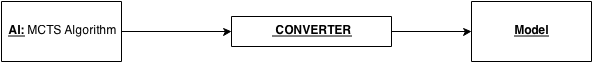
\includegraphics[width=0.80\textwidth]{2General_Architecture/2.2API/img/CONVERTER.png}
	\caption{Block Diagram of Converter}
	\label{fig:flowchart}
\end{figure}
\thispagestyle{empty}

